
% Template for Elsevier CRC journal article
% version 1.2 dated 09 May 2011

% This file (c) 2009-2011 Elsevier Ltd.  Modifications may be freely made,
% provided the edited file is saved under a different name

% This file contains modifications for Procedia Computer Science

% Changes since version 1.1
% - added "procedia" option compliant with ecrc.sty version 1.2a
%   (makes the layout approximately the same as the Word CRC template)
% - added example for generating copyright line in abstract

%-----------------------------------------------------------------------------------

%% This template uses the elsarticle.cls document class and the extension package ecrc.sty
%% For full documentation on usage of elsarticle.cls, consult the documentation "elsdoc.pdf"
%% Further resources available at http://www.elsevier.com/latex

%-----------------------------------------------------------------------------------

%%%%%%%%%%%%%%%%%%%%%%%%%%%%%%%%%%%%%%%%%%%%%%%%%%%%%%%%%%%%%%
%%%%%%%%%%%%%%%%%%%%%%%%%%%%%%%%%%%%%%%%%%%%%%%%%%%%%%%%%%%%%%
%%                                                          %%
%% Important note on usage                                  %%
%% -----------------------                                  %%
%% This file should normally be compiled with PDFLaTeX      %%
%% Using standard LaTeX should work but may produce clashes %%
%%                                                          %%
%%%%%%%%%%%%%%%%%%%%%%%%%%%%%%%%%%%%%%%%%%%%%%%%%%%%%%%%%%%%%%
%%%%%%%%%%%%%%%%%%%%%%%%%%%%%%%%%%%%%%%%%%%%%%%%%%%%%%%%%%%%%%

%% The '3p' and 'times' class options of elsarticle are used for Elsevier CRC
%% The 'procedia' option causes ecrc to approximate to the Word template
\documentclass[3p,times,procedia]{elsarticle}

%% The `ecrc' package must be called to make the CRC functionality available
\usepackage{ecrc}

%% The ecrc package defines commands needed for running heads and logos.
%% For running heads, you can set the journal name, the volume, the starting page and the authors

%% set the volume if you know. Otherwise `00'
\volume{00}

%% set the starting page if not 1
\firstpage{1}

%% Give the name of the journal
\journalname{Procedia Computer Science}

%% Give the author list to appear in the running head
%% Example \runauth{C.V. Radhakrishnan et al.}
\runauth{Ying Liu, Chao Xiang}

%% The choice of journal logo is determined by the \jid and \jnltitlelogo commands.
%% A user-supplied logo with the name <\jid>logo.pdf will be inserted if present.
%% e.g. if \jid{yspmi} the system will look for a file yspmilogo.pdf
%% Otherwise the content of \jnltitlelogo will be set between horizontal lines as a default logo

%% Give the abbreviation of the Journal.
\jid{procs}

%% Give a short journal name for the dummy logo (if needed)
\jnltitlelogo{Procedia Computer Science}

%% Provide the copyright line to appear in the abstract
%% Usage:
%   \CopyrightLine[<text-before-year>]{<year>}{<restt-of-the-copyright-text>}
%   \CopyrightLine[Crown copyright]{2011}{Published by Elsevier Ltd.}
%   \CopyrightLine{2011}{Elsevier Ltd. All rights reserved}
\CopyrightLine{2016}{The Authors. Published by Elsevier B.V.\newline Selection and/or peer-review under responsibility of ITQM2016}


%% Hereafter the template follows `elsarticle'.
%% For more details see the existing template files elsarticle-template-harv.tex and elsarticle-template-num.tex.

%% Elsevier CRC generally uses a numbered reference style
%% For this, the conventions of elsarticle-template-num.tex should be followed (included below)
%% If using BibTeX, use the style file elsarticle-num.bst

%% End of ecrc-specific commands
%%%%%%%%%%%%%%%%%%%%%%%%%%%%%%%%%%%%%%%%%%%%%%%%%%%%%%%%%%%%%%%%%%%%%%%%%%

%% The amssymb package provides various useful mathematical symbols
\usepackage{amssymb}
%% The amsthm package provides extended theorem environments
%% \usepackage{amsthm}

%% The lineno packages adds line numbers. Start line numbering with
%% \begin{linenumbers}, end it with \end{linenumbers}. Or switch it on
%% for the whole article with \linenumbers after \end{frontmatter}.
%% \usepackage{lineno}

%% natbib.sty is loaded by default. However, natbib options can be
%% provided with \biboptions{...} command. Following options are
%% valid:

%%   round  -  round parentheses are used (default)
%%   square -  square brackets are used   [option]
%%   curly  -  curly braces are used      {option}
%%   angle  -  angle brackets are used    <option>
%%   semicolon  -  multiple citations separated by semi-colon
%%   colon  - same as semicolon, an earlier confusion
%%   comma  -  separated by comma
%%   numbers-  selects numerical citations
%%   super  -  numerical citations as superscripts
%%   sort   -  sorts multiple citations according to order in ref. list
%%   sort&compress   -  like sort, but also compresses numerical citations
%%   compress - compresses without sorting
%%
%% \biboptions{comma,round}

% \biboptions{}

% if you have landscape tables
\usepackage[figuresright]{rotating}

% put your own definitions here:
%   \newcommand{\cZ}{\cal{Z}}
%   \newtheorem{def}{Definition}[section]
%   ...

% add words to TeX's hyphenation exception list
%\hyphenation{author another created financial paper re-commend-ed Post-Script}

% declarations for front matter

\begin{document}

\begin{frontmatter}

%% Title, authors and addresses

%% use the tnoteref command within \title for footnotes;
%% use the tnotetext command for the associated footnote;
%% use the fnref command within \author or \address for footnotes;
%% use the fntext command for the associated footnote;
%% use the corref command within \author for corresponding author footnotes;
%% use the cortext command for the associated footnote;
%% use the ead command for the email address,
%% and the form \ead[url] for the home page:
%%
%% \title{Title\tnoteref{label1}}
%% \tnotetext[label1]{}
%% \author{Name\corref{cor1}\fnref{label2}}
%% \ead{email address}
%% \ead[url]{home page}
%% \fntext[label2]{}
%% \cortext[cor1]{}
%% \address{Address\fnref{label3}}
%% \fntext[label3]{}

\dochead{Information Technology and Quantitative Management (ITQM 2016)}
%% Use \dochead if there is an article header, e.g. \dochead{Short communication}
%% \dochead can also be used to include a conference title, if directed by the editors
%% e.g. \dochead{17th International Conference on Dynamical Processes in Excited States of Solids}

\title{Hybrid learning net: a novel architecture for fast learning}

%% use optional labels to link authors explicitly to addresses:
%% \author[label1,label2]{<author name>}
%% \address[label1]{<address>}
%% \address[label2]{<address>}

\author[a]{Ying Liu}
\author[a]{Chao Xiang}

\address[a]{University of Chinese Academy of Sciences, Beijing 100049, China}

\begin{abstract}
%% Text of abstract
Currently, neural networks have 
succeeded in object recognition 
tasks based on images, natural 
language translation, and voice 
recognition, to name a few. 
However, neural nets are customly 
built for different applications 
and vary a lot in achitectures 
and model hyperparameters like 
learning rate and parameter 
initialization, what's worse,
these hyperparameter settings 
generally play a big role in 
performances of training and 
testing, and the best settings 
for specific applications are so 
far only available by manually 
repeatly trying different 
configurations which is really 
huge work. We, thereby, present 
a novel neural network achitecture,
called Hybrid Learning Net($\mathbf{HLN}$), 
with Self Organizing Maps(SOMs) 
embedded in each layer to learn 
from samples in $\mathbf{both}$ 
unsupervised and supervised way, 
targeting to achieve a much
$\mathbf{faster}$ net learning for general 
applications with $\mathbf{good}$ robustness
to a few key hyperparameters such 
as the parameter initialization
and the net strcuture variation. 
We've also experimented our 
architecture over the MNIST 
dataset, it has proved the 
impressive improvement on both 
training and testing phases
of general applications, 
say compared to the traditional
architecture, our method speed up
the training process by up to 
$\mathbf{40}$ times, which only
take $\mathbf{1}$ epoch to get 
an testing accuracy of over
$\mathbf{87.5\%}$, and takes
no more than $\mathbf{3}$ epoches
to reach a profound accuracy of 
over $\mathbf{91.3\%}$.
In addition, on big scale
of input dimension and/or with deeper 
architecture, where the traditional
architecture fails to learn at all,
our method still have a fast learning,
and can retrieve the same testing 
accuracy on MNIST.
Moreover, we have discovered 
some interesting facts about 
neural network trainings, 
such as neuron activation 
sparsity is strongly 
correlated to the training loss 
within certain cases which may shed 
a little light on how such 
architecture really works.
\end{abstract}

\begin{keyword}
hybrid learning; neural network; general application; sparsity; SOM; MNIST; fast learning

%% keywords here, in the form: keyword \sep keyword

%% PACS codes here, in the form: \PACS code \sep code

%% MSC codes here, in the form: \MSC code \sep code
%% or \MSC[2008] code \sep code (2000 is the default)

\end{keyword}

\end{frontmatter}

\correspondingauthor[*]{Corresponding author. Tel.: +86-183-0114-2368;}
\email{xiangchao215@mails.ucas.ac.cn}

%%
%% Start line numbering here if you want
%%
% \linenumbers

%% main text
\section{Introduction}
\label{main}
Since the first mathematical model 
of artificial neural network was 
proposed in 1943\cite{mcculloch1943logical}, 
the neural network has been 
designed into many architectures, 
such as Convolutional Neural 
Networks(CNNs) for image 
recognition
\cite{krizhevsky2012imagenet}, 
Recurrent Convolutional Neural 
Networks(R-CNNs) for object 
detection in 
videos\cite{girshick2015fast}, 
and Long Short Term Memorys(LSTMs)
for speech recognition
\cite{graves2013hybrid} and many, 
many more to make it a list. 
These specially designed neural 
network models are trained by 
lots of efficient methods with 
tons of carefully chosen little 
skills which we may call tricks. 
Such neural network architectures
suit well for their specific 
applications but may have plain 
or worse performances on others, 
and their best performances 
rely heavily on hyperparameter 
configuration in general. Thus, 
it is an in-demand job to propose 
a relatively universal 
architecutre that enables equal 
or similar performances among 
varied applications.

We notice that, although there're 
plenty of choices to train a 
neural network, literally all 
these methods can be reduced into
3 categories, supervised learning
\cite{lecun1990handwritten}, 
unsupervised learning
\cite{vincent2010stacked}, 
and the semi-supervised
\cite{chapelle2009semi}.
In supervised learning, 
one can only train a model from 
labeled samples, however in real 
applications, labeling a large 
dataset is a tough and costly 
task, the unlabeled ones are 
therefore the primary data 
available. To make use of the 
majority unlabeled data, a few 
unsupervised training algorithms 
arose. These unsupervised learning
methods, denoted as pretraining, 
attempt to produce an optimized 
parameter initialization
\cite{le2013building}.
Thus such unsupervised techniques 
can only be applied before the 
supervised training phase, once 
the supervised begins, the 
unsupversied learning will become 
unavailable for the model.
While the semi-supervised learning
allows the model to learn from
both labeled and unlabeled samples 
at the same time, however they use a
regularizer to embed the semi-supervised
learner to original optimizing object,
and generally a balance constraint is
required to avoid the trival solution
\cite{socher2011semi}.
Such a enhanced learner brings more 
hyperparameters(say the balance 
constraint), making it even more 
difficult to search for best settings
for current architectures. 
Additionally, this integration way 
makes it impossible to separate the 
two learners as the semi-supervised 
regularizer is built on the supervised 
learner, and therefore requires an 
early supervised training alone with 
profound labeled data before the 
semi-supervised regularizer can be
applied.
Thus we introduce a new architecture
that learn in both supervised and 
unsupervised ways at the same time,
and requires no extra techniques on
training. Our architecture, Hybrid
Learning Nets(HLNs), made of 
stacked layers, with each hidden
layer embedded with a Self Organizing
Map(SOM), training in
the simplest way of backprop, 
demonstrate much faster learning
capability and remain robust to 
parameter initialization and
network configuration such as the net
depth of layer.

%\subsection{Our contributes}
The main contributions of our work are:
\begin{itemize}
\item We propose HLN, a SOM-embedded 
architecture to learn both unlabeled 
and labeled data at the same time.
\item Our architecture HLN overcomes
the problem brought by traditional 
semi-supervised learning methods that 
the semi-supervised learning requires
an early standalone training for the
supervised learner which contradicts
with the key condition: no enough 
labeled data is provided.
\item The HLN uses a SOM embedding 
coupling the first hidden layer near 
to the input layer, to learn a cluster 
mapping function from the cheap and 
massive unlabeled data, and this process
can occur at any time, no matter the 
supervised learning begins or not,
they're completely separated.
For deeper hidden layers, each of them 
also has a SOM-embedding coupled, 
but can only learn from labeled data.
\item The experimental result shows HLNs
speed up the whole training a lot.
\item Our architecture demonstrates a 
good robustness to some hyperparameters
which may slightly relax the work of 
manually searching for best settings
of hyperparameters by repeatly trying
different configurations and run the
whole training and testing over and 
over again.
\end{itemize}
HLN is implemented in Python and all
our code and results of experiments
in detail are available at 
\cololinks{https://github.com/hiroki-kyoto/hybrid-learning-net.git}

%\subsection{The organization of this artical}



\section{Related work}

\subsection{Semi-supervised learning for
neural network}
A key assumption in semi-supervised 
algorithms developed so far, is the 
structure assumption: two samples with 
similar distribution on the same mapping 
structure tend to have high probability 
of belonging to the same class. Based on 
this assumption, one can use large 
unlabeled data to uncover such 
structures. There're already a few 
algorithms dedicated to do this,
such as cluster kernels
\cite{chapelle2003cluster},
Low Density Separation(LDS)
\cite{chapelle2005semi},
label propagation
\cite{zhu2002learning},
to name a few.
In such algorithms, designing a regularizer
to enable the model to learn the representation
or structure of raw data, in order to improve
the supervised learning performance, becomes
the key point.

To get a clear idea of how such semi-supervised
learning algorithms work, we will give a brief 
recall to some.
Let's firstly focus on the general algorithm
description of semi-supervised learning.
Given a set of unlabeled samples,
$\mathbf{X}=\{x_1,\cdots,x_N\}
(x\in\mathbb{R}^d)$,
and the similarity labels between any
$x_i$ and $x_j$,
$\mathbf{W}=\{W_{ij}|i,j=1,\cdots,N\}$,
we're to find the best embedding function, 
$f(x)$, for each sample $x_i$, to minimize:
\begin{equation}
\sum^{N}_{i=1}\sum^{N}_{j=1}L(f(x_i),f(x_j),W_{ij})
\label{eq:1}
\end{equation}

to explain it,
\begin{itemize}[]
\item $L(\cdot)$ is the loss function of 3 variables: 
$\left<f(x_i),f(x_j),W_{ij}\right>$, 
such as 
$$L(f(x_i),f(x_j),W_{ij}) = 
\max(0,||f(x_i)-f(x_j)||-W_{ij})$$
\item $f(x)\in\mathbb{R}^n$ is the embedding function, it tries to produce
a vector from $x_i$, similar to that of $x_j$ with $W_{ij}=0$,
and disimilar with $W_{ij}=1$.
\item $W_{ij}\in \mathbb{R}$ is the similarity label of the sample pair
$\left<x_i,x_j\right>$ from $\mathbf{X}$.
\end{itemize}



\subsection{ Tables}

All tables should be numbered with Arabic numerals. Headings should be placed above tables, left justified. Leave one line space between the heading and the table. Only horizontal lines should be used within a table, to distinguish the column headings from the body of the table, and immediately above and below the table. Tables must be embedded into the text and not supplied separately. Below is an example which authors may find useful.

\begin{table}[h]
\caption{An example of a table.}
\begin{tabular*}{\hsize}{@{\extracolsep{\fill}}lll@{}}
\hline
An example of a column heading & Column A (t) & Column B (T)\\
\hline
And an entry &   1 &  2\\
And another entry  & 3 &  4\\
And another entry &  5 &  6\\
\hline
\end{tabular*}
\end{table}


\subsection{ Construction of references}

References should be added at the end of the paper, and its corresponding citation will be added in the order of their appearance in the text. Authors should ensure that every reference in the text appears in the list of references and vice versa. Indicate references by [1], [2-3] in the text. The actual authors can be referred to, but the reference citation(s) must always be given. Some examples of how your references should be listed are given at the end of this template in the `References' section, which will allow you to assemble your reference list according to the correct format and font size.

\subsection{Section headings}
Section headings should be left justified, with the first letter capitalized and numbered consecutively, starting with the Introduction. Sub-section headings should be in capital and lower-case italic letters, numbered 1.1, 1.2, etc, and left justified, with second and subsequent lines indented. You may need to insert a page break to keep a heading with its text.

\subsection{General guidelines for the preparation of your text}
Avoid hyphenation at the end of a line. Symbols denoting vectors and matrices should be indicated in bold type. Scalar variable names should normally be expressed using italics. Weights and measures should be expressed in SI units. Please title your files in this order conferenceacrynom\_authorslastname.pdf


\section{SOMs-embedding for deep architecture}
A recall to SOMs.

How we construct deep architecture with SOMs-embeddings.

\section{Empirical Study}
To test our architecture performance on small data, we 
use a synthetic dataset containing $3.5\%$ noisy samples. 
A sampling from this dataset get the

\begin{figure}[h]
\centerline{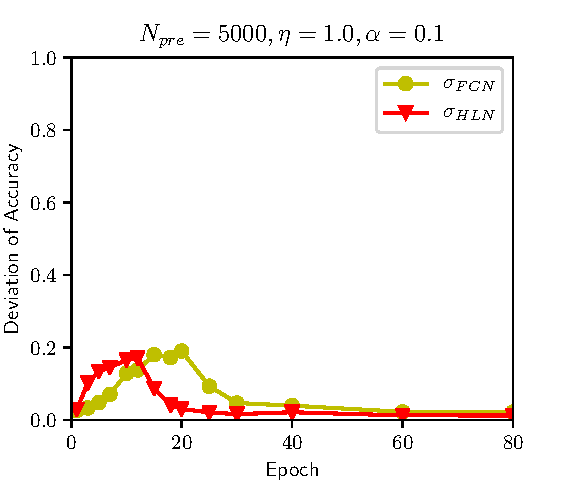
\includegraphics{fx1}\hspace*{5mm}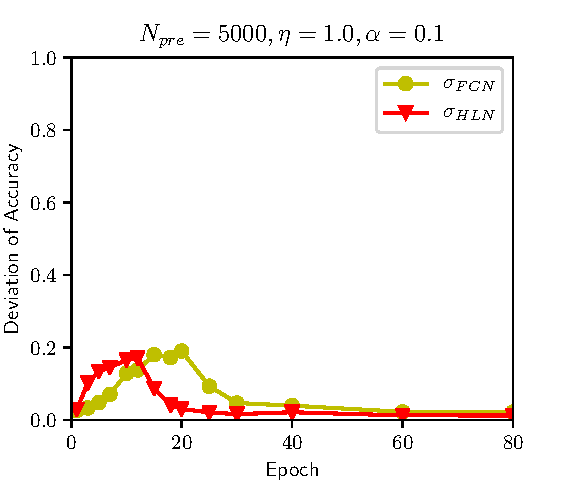
\includegraphics{fx1}}
\caption{(a) first picture; (b) second picture.}
\end{figure}


The figure number and caption should be typed below the illustration in 8 pt and left justified. For more guidelines and information to help you submit high quality artwork please visit: http://www.elsevier.comwps/find/authorsview. authors/authorartworkinstructions. Artwork has no text along the side of it in the main body of the text. However, if two images fit next to each other, these may be placed next to each other to save space, see Fig 1. They must be numbered consecutively, all figures, and all tables respectively.


\subsection{Footnotes}
Footnotes should be avoided if possible. Necessary footnotes should be denoted in the text by consecutive superscript letters. The footnotes should be typed single spaced, and in smaller type size (8 pt), at the foot of the page in which they are mentioned, and separated from the main text by a short line extending at the foot of the column. The `Els-footnote' style is available in this template for the text of the footnote.

Equations and formulae should be typed and numbered consecutively with Arabic numerals in parentheses on the right hand side of the page (if referred to explicitly in the text),
\begin{equation}
\begin{array}{rcl}
\displaystyle X_r &=& \displaystyle\dot{Q}^{"}_{rad}\left/\left(\dot{Q}^{"}_{rad} + \dot{Q}^{"}_{conv}\right)\right.\\[6pt]
\displaystyle \rho &=& \displaystyle\frac{\vec{E}}{J_c(T={\rm const.})\cdot\left(P\cdot\left(\displaystyle\frac{\vec{E}}{E_c}\right)^m+(1-P)\right)}
\end{array}
\end{equation}

They should also be separated from the surrounding text by one space.

\section{Online licence}
All authors must Transfer the Online licence before the article can be published. This transfer agreement enables Elsevier to protect the copyrighted material for the authors, but does not relinquish the authors' proprietary rights. The copyright transfer covers the exclusive rights to reproduce and distribute the article, including reprints, photographic reproductions, microfilm or any other reproductions of similar nature and translations. Authors are responsible for obtaining from the copyright holder permission to reproduce any figures for which copyright exists.


The citation must be used in following style: \cite{article-minimal}, \cite{article-full}, \cite{article-crossref}, \cite{whole-journal} and \cite{inbook-minimal}.

\section*{Acknowledgements}

These and the Reference headings are in bold but have no numbers. Text below continues as normal.

%% References
%%
%% Following citation commands can be used in the body text:
%% Usage of \cite is as follows:
%%   \cite{key}         ==>>  [#]
%%   \cite[chap. 2]{key} ==>> [#, chap. 2]
%%


%% References with BibTeX database:

\bibliographystyle{elsarticle-num}
\bibliography{ref}

%% Authors are advised to use a BibTeX database file for their reference list.
%% The provided style file elsarticle-num.bst formats references in the required Procedia style

%% For references without a BibTeX database:

% \begin{thebibliography}{00}

%% \bibitem must have the following form:
%%   \bibitem{key}...
%%

% \bibitem{}

% \end{thebibliography}


%% The Appendices part is started with the command \appendix;
%% appendix sections are then done as normal sections
%% \appendix

%% \section{}
%% \label{}

\appendix
\section{An example appendix}
Authors including an appendix section should do so after References section. Multiple appendices should all have headings in the style used above. They will automatically be ordered A, B, C etc.

\subsection{Example of a sub-heading within an appendix}
There is also the option to include a subheading within the Appendix if you wish.

\end{document}

%%
%% End of file `procs-template.tex'.
